% Options for packages loaded elsewhere
\PassOptionsToPackage{unicode}{hyperref}
\PassOptionsToPackage{hyphens}{url}
%
\documentclass[
]{article}
\usepackage{amsmath,amssymb}
\usepackage{lmodern}
\usepackage{iftex}
\ifPDFTeX
  \usepackage[T1]{fontenc}
  \usepackage[utf8]{inputenc}
  \usepackage{textcomp} % provide euro and other symbols
\else % if luatex or xetex
  \usepackage{unicode-math}
  \defaultfontfeatures{Scale=MatchLowercase}
  \defaultfontfeatures[\rmfamily]{Ligatures=TeX,Scale=1}
\fi
% Use upquote if available, for straight quotes in verbatim environments
\IfFileExists{upquote.sty}{\usepackage{upquote}}{}
\IfFileExists{microtype.sty}{% use microtype if available
  \usepackage[]{microtype}
  \UseMicrotypeSet[protrusion]{basicmath} % disable protrusion for tt fonts
}{}
\makeatletter
\@ifundefined{KOMAClassName}{% if non-KOMA class
  \IfFileExists{parskip.sty}{%
    \usepackage{parskip}
  }{% else
    \setlength{\parindent}{0pt}
    \setlength{\parskip}{6pt plus 2pt minus 1pt}}
}{% if KOMA class
  \KOMAoptions{parskip=half}}
\makeatother
\usepackage{xcolor}
\usepackage[margin=1in]{geometry}
\usepackage{longtable,booktabs,array}
\usepackage{calc} % for calculating minipage widths
% Correct order of tables after \paragraph or \subparagraph
\usepackage{etoolbox}
\makeatletter
\patchcmd\longtable{\par}{\if@noskipsec\mbox{}\fi\par}{}{}
\makeatother
% Allow footnotes in longtable head/foot
\IfFileExists{footnotehyper.sty}{\usepackage{footnotehyper}}{\usepackage{footnote}}
\makesavenoteenv{longtable}
\usepackage{graphicx}
\makeatletter
\def\maxwidth{\ifdim\Gin@nat@width>\linewidth\linewidth\else\Gin@nat@width\fi}
\def\maxheight{\ifdim\Gin@nat@height>\textheight\textheight\else\Gin@nat@height\fi}
\makeatother
% Scale images if necessary, so that they will not overflow the page
% margins by default, and it is still possible to overwrite the defaults
% using explicit options in \includegraphics[width, height, ...]{}
\setkeys{Gin}{width=\maxwidth,height=\maxheight,keepaspectratio}
% Set default figure placement to htbp
\makeatletter
\def\fps@figure{htbp}
\makeatother
\setlength{\emergencystretch}{3em} % prevent overfull lines
\providecommand{\tightlist}{%
  \setlength{\itemsep}{0pt}\setlength{\parskip}{0pt}}
\setcounter{secnumdepth}{-\maxdimen} % remove section numbering
\ifLuaTeX
  \usepackage{selnolig}  % disable illegal ligatures
\fi
\IfFileExists{bookmark.sty}{\usepackage{bookmark}}{\usepackage{hyperref}}
\IfFileExists{xurl.sty}{\usepackage{xurl}}{} % add URL line breaks if available
\urlstyle{same} % disable monospaced font for URLs
\hypersetup{
  pdftitle={Meta-análises},
  pdfauthor={Clarissa F. D. Carneiro},
  hidelinks,
  pdfcreator={LaTeX via pandoc}}

\title{Meta-análises}
\author{Clarissa F. D. Carneiro}
\date{2022-10-18}

\begin{document}
\maketitle

\begin{verbatim}
## Warning: Paket 'readxl' wurde unter R Version 4.1.3 erstellt
\end{verbatim}

\begin{verbatim}
## Warning: Paket 'tidyverse' wurde unter R Version 4.1.3 erstellt
\end{verbatim}

\begin{verbatim}
## -- Attaching packages --------------------------------------- tidyverse 1.3.2 --
## v ggplot2 3.4.0      v purrr   1.0.0 
## v tibble  3.1.8      v dplyr   1.0.10
## v tidyr   1.2.1      v stringr 1.5.0 
## v readr   2.1.3      v forcats 0.5.2
\end{verbatim}

\begin{verbatim}
## Warning: Paket 'ggplot2' wurde unter R Version 4.1.3 erstellt
\end{verbatim}

\begin{verbatim}
## Warning: Paket 'tibble' wurde unter R Version 4.1.3 erstellt
\end{verbatim}

\begin{verbatim}
## Warning: Paket 'tidyr' wurde unter R Version 4.1.3 erstellt
\end{verbatim}

\begin{verbatim}
## Warning: Paket 'readr' wurde unter R Version 4.1.3 erstellt
\end{verbatim}

\begin{verbatim}
## Warning: Paket 'purrr' wurde unter R Version 4.1.3 erstellt
\end{verbatim}

\begin{verbatim}
## Warning: Paket 'dplyr' wurde unter R Version 4.1.3 erstellt
\end{verbatim}

\begin{verbatim}
## Warning: Paket 'stringr' wurde unter R Version 4.1.3 erstellt
\end{verbatim}

\begin{verbatim}
## Warning: Paket 'forcats' wurde unter R Version 4.1.3 erstellt
\end{verbatim}

\begin{verbatim}
## -- Conflicts ------------------------------------------ tidyverse_conflicts() --
## x dplyr::filter() masks stats::filter()
## x dplyr::lag()    masks stats::lag()
\end{verbatim}

\begin{verbatim}
## Warning: Paket 'metafor' wurde unter R Version 4.1.3 erstellt
\end{verbatim}

\begin{verbatim}
## Lade nötiges Paket: Matrix
\end{verbatim}

\begin{verbatim}
## Warning: Paket 'Matrix' wurde unter R Version 4.1.3 erstellt
\end{verbatim}

\begin{verbatim}
## 
## Attache Paket: 'Matrix'
## 
## Die folgenden Objekte sind maskiert von 'package:tidyr':
## 
##     expand, pack, unpack
## 
## Lade nötiges Paket: metadat
## 
## Loading the 'metafor' package (version 3.8-1). For an
## introduction to the package please type: help(metafor)
\end{verbatim}

\begin{verbatim}
## Warning: Paket 'metaviz' wurde unter R Version 4.1.3 erstellt
\end{verbatim}

\begin{verbatim}
## Warning: Paket 'glmulti' wurde unter R Version 4.1.3 erstellt
\end{verbatim}

\begin{verbatim}
## Lade nötiges Paket: rJava
## Lade nötiges Paket: leaps
\end{verbatim}

\begin{verbatim}
## Warning: Paket 'leaps' wurde unter R Version 4.1.3 erstellt
\end{verbatim}

\begin{verbatim}
## Warning: Paket 'knitr' wurde unter R Version 4.1.3 erstellt
\end{verbatim}

Depois da limpeza, importamos de volta para análises.

\begin{verbatim}
## Warning: Coercing text to numeric in AP1025 / R1025C42: '100.0'
\end{verbatim}

\begin{verbatim}
## Warning: Coercing text to numeric in AP1026 / R1026C42: '100.0'
\end{verbatim}

\begin{verbatim}
## Warning: Coercing text to numeric in AP1027 / R1027C42: '100.0'
\end{verbatim}

\begin{verbatim}
## Warning: Coercing text to numeric in AP1028 / R1028C42: '100.0'
\end{verbatim}

\begin{verbatim}
## Warning: Coercing text to numeric in AP1029 / R1029C42: '100.0'
\end{verbatim}

\begin{verbatim}
## Warning: Coercing text to numeric in AP1030 / R1030C42: '100.0'
\end{verbatim}

\begin{verbatim}
## Warning: Coercing text to numeric in AP1031 / R1031C42: '100.0'
\end{verbatim}

\begin{verbatim}
## Warning: Coercing text to numeric in AP1032 / R1032C42: '100.0'
\end{verbatim}

\begin{verbatim}
## Warning: Coercing text to numeric in AP1033 / R1033C42: '100.0'
\end{verbatim}

\begin{verbatim}
## Warning: Coercing text to numeric in AP1034 / R1034C42: '100.0'
\end{verbatim}

\begin{verbatim}
## Warning: Coercing text to numeric in AP1035 / R1035C42: '100.0'
\end{verbatim}

\begin{verbatim}
## Warning: Coercing text to numeric in AP1036 / R1036C42: '100.0'
\end{verbatim}

\begin{verbatim}
## Warning: Coercing text to numeric in AP1037 / R1037C42: '100.0'
\end{verbatim}

\begin{verbatim}
## Warning: Coercing text to numeric in AP1038 / R1038C42: '100.0'
\end{verbatim}

\begin{verbatim}
## Warning: Coercing text to numeric in AP1039 / R1039C42: '100.0'
\end{verbatim}

\begin{verbatim}
## Warning: Coercing text to numeric in AP1040 / R1040C42: '100.0'
\end{verbatim}

\begin{verbatim}
## Warning: Coercing text to numeric in AP1041 / R1041C42: '100.0'
\end{verbatim}

\begin{verbatim}
## Warning: Coercing text to numeric in AP1042 / R1042C42: '100.0'
\end{verbatim}

\begin{verbatim}
## Warning: Coercing text to numeric in AP1043 / R1043C42: '100.0'
\end{verbatim}

\begin{verbatim}
## Warning: Coercing text to numeric in AP1044 / R1044C42: '100.0'
\end{verbatim}

\begin{verbatim}
## Warning: Coercing text to numeric in AP1045 / R1045C42: '100.0'
\end{verbatim}

\begin{verbatim}
## Warning: Coercing text to numeric in AP1046 / R1046C42: '100.0'
\end{verbatim}

\begin{verbatim}
## Warning: Coercing text to numeric in AP1047 / R1047C42: '100.0'
\end{verbatim}

\begin{verbatim}
## Warning: Coercing text to numeric in AP1048 / R1048C42: '100.0'
\end{verbatim}

\begin{verbatim}
## Warning: Coercing text to numeric in AP1049 / R1049C42: '100.0'
\end{verbatim}

\begin{verbatim}
## Warning: Coercing text to numeric in AP1050 / R1050C42: '100.0'
\end{verbatim}

\begin{verbatim}
## Warning: Coercing text to numeric in AP1051 / R1051C42: '100.0'
\end{verbatim}

\begin{verbatim}
## Warning: Coercing text to numeric in AP1052 / R1052C42: '100.0'
\end{verbatim}

\begin{verbatim}
## Warning: Coercing text to numeric in AP1053 / R1053C42: '100.0'
\end{verbatim}

\begin{verbatim}
## Warning: Coercing text to numeric in AP1054 / R1054C42: '100.0'
\end{verbatim}

\begin{verbatim}
## Warning: Coercing text to numeric in AP1055 / R1055C42: '100.0'
\end{verbatim}

\begin{verbatim}
## Warning: Coercing text to numeric in AP1056 / R1056C42: '100.0'
\end{verbatim}

\begin{verbatim}
## Warning: Coercing text to numeric in AP1057 / R1057C42: '100.0'
\end{verbatim}

\begin{verbatim}
## Warning: Coercing text to numeric in AP1058 / R1058C42: '100.0'
\end{verbatim}

\begin{verbatim}
## Warning: Coercing text to numeric in AP1059 / R1059C42: '100.0'
\end{verbatim}

\begin{verbatim}
## Warning: Coercing text to numeric in AP1060 / R1060C42: '100.0'
\end{verbatim}

\begin{verbatim}
## Warning: Coercing text to numeric in AP1061 / R1061C42: '100.0'
\end{verbatim}

\begin{verbatim}
## Warning: Coercing text to numeric in AP1062 / R1062C42: '100.0'
\end{verbatim}

\begin{verbatim}
## Warning: Coercing text to numeric in AP1063 / R1063C42: '100.0'
\end{verbatim}

\begin{verbatim}
## Warning: Coercing text to numeric in AP1064 / R1064C42: '100.0'
\end{verbatim}

\begin{verbatim}
## Warning: Coercing text to numeric in AP1065 / R1065C42: '100.0'
\end{verbatim}

\begin{verbatim}
## Warning: Coercing text to numeric in AP1066 / R1066C42: '100.0'
\end{verbatim}

\begin{verbatim}
## Warning: Coercing text to numeric in AP1067 / R1067C42: '100.0'
\end{verbatim}

\begin{verbatim}
## Warning: Coercing text to numeric in AP1068 / R1068C42: '100.0'
\end{verbatim}

\begin{verbatim}
## Warning: Coercing text to numeric in AP1069 / R1069C42: '100.0'
\end{verbatim}

\begin{verbatim}
## Warning: Coercing text to numeric in AP1070 / R1070C42: '100.0'
\end{verbatim}

\begin{verbatim}
## Warning: Coercing text to numeric in AP1071 / R1071C42: '100.0'
\end{verbatim}

\begin{verbatim}
## Warning: Coercing text to numeric in AP1072 / R1072C42: '100.0'
\end{verbatim}

\begin{verbatim}
## Warning: Coercing text to numeric in AP1073 / R1073C42: '100.0'
\end{verbatim}

\begin{verbatim}
## Warning: Coercing text to numeric in AP1074 / R1074C42: '100.0'
\end{verbatim}

\begin{verbatim}
## Warning: Coercing text to numeric in AP1075 / R1075C42: '100.0'
\end{verbatim}

\begin{verbatim}
## Warning: Coercing text to numeric in AP1076 / R1076C42: '100.0'
\end{verbatim}

\begin{verbatim}
## Warning: Expecting numeric in S1642 / R1642C19: got '95.770; 79.780; 89.150;
## 100.200; 105.100; 96.320; 102.400'
\end{verbatim}

\begin{verbatim}
## Warning: Expecting numeric in T1642 / R1642C20: got '2.022; 4.228; 5.331; 2.390;
## 2.757; 4.044; 3.125'
\end{verbatim}

Para análises, precisamos da média e n dos dois grupos e da variacao no
tratado, seja SEM, SD ou Unclear. Também precisamos excluir casos em que
a sequencia de abeta nao esteja clara.

Para montar um fluxograma: Número de comparações extraídas = 1664 Número
de comparações excluídas por falta de dados = 470

Outras limpezas:

Calculei SDs a partir de SEMs (se estava `unclear', considerei SEM).

Para usar SMD, precisamos do SD dos dois grupos necessariamente -
decidimos considerar sd do controle igual ao tratado (que vai ser igual
ao pooled), pelo menos até Olavo revisar artigos sobre o assunto.

Meta-análise (2-level SMD)

\begin{verbatim}
## Warning: Studies with NAs omitted from model fitting.
\end{verbatim}

\begin{verbatim}
## Warning: Ratio of largest to smallest sampling variance extremely large. May not
## be able to obtain stable results.
\end{verbatim}

\begin{verbatim}
## 
## Random-Effects Model (k = 1188; tau^2 estimator: REML)
## 
##     logLik    deviance         AIC         BIC        AICc   
## -3791.7823   7583.5646   7587.5646   7597.7230   7587.5748   
## 
## tau^2 (estimated amount of total heterogeneity): 12.9046 (SE = 0.6670)
## tau (square root of estimated tau^2 value):      3.5923
## I^2 (total heterogeneity / total variability):   92.07%
## H^2 (total variability / sampling variability):  12.62
## 
## Test for Heterogeneity:
## Q(df = 1187) = 7172.3259, p-val < .0001
## 
## Model Results:
## 
## estimate      se      zval    pval    ci.lb    ci.ub      
##  -4.7325  0.1197  -39.5492  <.0001  -4.9671  -4.4980  *** 
## 
## ---
## Signif. codes:  0 '***' 0.001 '**' 0.01 '*' 0.05 '.' 0.1 ' ' 1
\end{verbatim}

Sobre o alerta ``Ratio of largest to smallest sampling variance
extremely large. May not be able to obtain stable results.'', ver essa
discussao:
\url{https://stat.ethz.ch/pipermail/r-sig-meta-analysis/2019-February/001426.html}
Podemos conferir a distribuicao de sample sizes e de vi para ver onde
pode estar o problema:

\begin{verbatim}
##    Min. 1st Qu.  Median    Mean 3rd Qu.    Max. 
##   1.000   3.000   3.000   4.216   4.000  24.000
\end{verbatim}

\begin{verbatim}
##    Min. 1st Qu.  Median    Mean 3rd Qu.    Max. 
##    1.00    3.00    3.00    4.22    4.00   24.00
\end{verbatim}

\begin{verbatim}
##      Min.   1st Qu.    Median      Mean   3rd Qu.      Max.      NA's 
##       0.1       0.8       2.3    1489.0       6.9 1494773.7         6
\end{verbatim}

\begin{longtable}[]{@{}lrr@{}}
\toprule()
rayyan.key & yi & vi \\
\midrule()
\endhead
rayyan-115935411 & -3458.06035 & 1494773.6746 \\
rayyan-115935411 & -900.85105 & 101442.5762 \\
rayyan-115922365 & 1158.08205 & 83822.6278 \\
rayyan-115923162 & -920.56888 & 70621.2546 \\
rayyan-115935519 & -156.71039 & 2047.1788 \\
rayyan-115934663 & -167.47123 & 1753.4132 \\
rayyan-115922941 & -114.15348 & 1086.5848 \\
rayyan-115934780 & -91.29182 & 695.1830 \\
rayyan-115922941 & -82.20311 & 563.7792 \\
rayyan-115926424 & -141.59031 & 501.3954 \\
\bottomrule()
\end{longtable}

\begin{longtable}[]{@{}lrr@{}}
\toprule()
rayyan.key & yi & vi \\
\midrule()
\endhead
rayyan-115928295 & -0.3530388 & 0.1015580 \\
rayyan-115928431 & -0.7329931 & 0.1016343 \\
rayyan-115928431 & -0.8843718 & 0.1045490 \\
rayyan-115928431 & -0.9461367 & 0.1058949 \\
rayyan-115928431 & -1.0620553 & 0.1086662 \\
rayyan-115928431 & -1.1683500 & 0.1114886 \\
rayyan-115928431 & -1.2023444 & 0.1124480 \\
rayyan-115921714 & -0.3598424 & 0.1129095 \\
rayyan-115928431 & -1.2202264 & 0.1129637 \\
rayyan-115928431 & -1.2354837 & 0.1134098 \\
\bottomrule()
\end{longtable}

Além desses casos, observamos também outras comparacoes com tamanhos de
efeito muito extremos. Devemos conferir esses outliers, comecando pelos
mais extremos. Dependendo de quantos erros encontrarmos, decidimos até
que threshold deveríamos conferir todas as extracoes.

\begin{longtable}[]{@{}lrr@{}}
\toprule()
rayyan.key & yi & vi \\
\midrule()
\endhead
rayyan-115935411 & -3458.0604 & 1494773.6746 \\
rayyan-115923162 & -920.5689 & 70621.2546 \\
rayyan-115935411 & -900.8510 & 101442.5762 \\
rayyan-115934663 & -167.4712 & 1753.4132 \\
rayyan-115935519 & -156.7104 & 2047.1788 \\
rayyan-115926424 & -141.5903 & 501.3954 \\
rayyan-115922941 & -114.1535 & 1086.5848 \\
\bottomrule()
\end{longtable}

\begin{longtable}[]{@{}lrr@{}}
\toprule()
rayyan.key & yi & vi \\
\midrule()
\endhead
rayyan-115934780 & -91.29182 & 695.18301 \\
rayyan-115934663 & -82.99467 & 431.00720 \\
rayyan-115922941 & -82.20311 & 563.77923 \\
rayyan-115926929 & -75.10359 & 353.03435 \\
rayyan-115934780 & -74.76896 & 466.53317 \\
rayyan-115926929 & -71.49641 & 319.98356 \\
rayyan-115926929 & -62.82952 & 247.22178 \\
rayyan-115922941 & -60.64623 & 307.16372 \\
rayyan-115934663 & -57.79245 & 209.24796 \\
rayyan-115922135 & -55.27814 & 85.10201 \\
\bottomrule()
\end{longtable}

\begin{longtable}[]{@{}lrr@{}}
\toprule()
rayyan.key & yi & vi \\
\midrule()
\endhead
rayyan-115931943 & -49.30428 & 203.242661 \\
rayyan-115934663 & -48.66451 & 148.514653 \\
rayyan-115927526 & -46.98657 & 92.322421 \\
rayyan-115934780 & -46.49493 & 180.814878 \\
rayyan-115926929 & -42.79691 & 114.973449 \\
rayyan-115925532 & -42.55829 & 151.600637 \\
rayyan-115922231 & -42.40337 & 150.503791 \\
rayyan-115935519 & -41.84040 & 146.551602 \\
rayyan-115931423 & -41.22825 & 142.314049 \\
rayyan-115926929 & -40.81236 & 104.603043 \\
rayyan-115925844 & -38.95400 & 127.117836 \\
rayyan-115935519 & -37.18481 & 115.892521 \\
rayyan-115925844 & -37.04514 & 115.028546 \\
rayyan-115923351 & -36.80108 & 113.526609 \\
rayyan-115924192 & -36.13161 & 65.674644 \\
rayyan-115931943 & -32.49122 & 88.639942 \\
rayyan-115935423 & -32.29988 & 87.606869 \\
rayyan-115924256 & -32.16434 & 130.318107 \\
rayyan-115935423 & -31.89760 & 85.454762 \\
rayyan-115922833 & -30.36920 & 77.524000 \\
rayyan-115921852 & -29.86821 & 75.009156 \\
rayyan-115933128 & -29.82300 & 74.784275 \\
rayyan-115921843 & -29.56424 & 31.501586 \\
rayyan-115924722 & -28.98891 & 35.348206 \\
rayyan-115922818 & -28.26534 & 40.346481 \\
rayyan-115935423 & -27.90157 & 65.541451 \\
rayyan-115922231 & -26.77816 & 60.422473 \\
rayyan-115927187 & -26.60799 & 59.665425 \\
rayyan-115931957 & -26.58102 & 44.659418 \\
rayyan-115931423 & -26.27171 & 58.183557 \\
rayyan-115924594 & -26.26370 & 58.148495 \\
rayyan-115930933 & -26.19636 & 57.854112 \\
rayyan-115923717 & -25.85791 & 28.192977 \\
rayyan-115921698 & -25.32565 & 54.115703 \\
rayyan-115933128 & -25.11911 & 53.247470 \\
rayyan-115936583 & -24.70093 & 25.755672 \\
rayyan-115927187 & -24.48598 & 50.630271 \\
rayyan-115936583 & -24.31967 & 24.976939 \\
rayyan-115925844 & -24.25832 & 49.705508 \\
rayyan-115933981 & -24.24713 & 37.245217 \\
rayyan-115922941 & -24.21650 & 49.536558 \\
rayyan-115925844 & -24.01692 & 48.734365 \\
rayyan-115924256 & -23.81655 & 71.903533 \\
rayyan-115932219 & -23.67300 & 47.367587 \\
rayyan-115924514 & -23.54966 & 46.882212 \\
rayyan-115931755 & -23.51236 & 46.735931 \\
rayyan-115927526 & -23.27369 & 22.902703 \\
rayyan-115922673 & -22.87720 & 33.210401 \\
rayyan-115922673 & -22.29643 & 31.570688 \\
rayyan-115924381 & -21.56554 & 39.422697 \\
rayyan-115934663 & -21.27654 & 28.793191 \\
rayyan-115931948 & -21.24102 & 9.566271 \\
rayyan-115936583 & -21.16561 & 18.999289 \\
rayyan-115922833 & -20.97763 & 37.338399 \\
rayyan-115925844 & -20.75693 & 36.570862 \\
rayyan-115932334 & -20.70387 & 36.387535 \\
rayyan-115931034 & -20.39043 & 35.314130 \\
rayyan-115923717 & -20.24854 & 17.416805 \\
rayyan-115931034 & -20.18452 & 34.617901 \\
rayyan-115925844 & -20.16701 & 34.559021 \\
rayyan-115936964 & -20.06532 & 34.218086 \\
rayyan-115924269 & -20.00731 & 34.024375 \\
\bottomrule()
\end{longtable}

\begin{longtable}[]{@{}lrr@{}}
\toprule()
rayyan.key & yi & vi \\
\midrule()
\endhead
rayyan-115931957 & -19.69403 & 24.740927 \\
rayyan-115922871 & -19.54096 & 32.487418 \\
rayyan-115925987 & -19.53141 & 32.456341 \\
rayyan-115923525 & -19.17059 & 15.646318 \\
rayyan-115928224 & -19.13376 & 46.762572 \\
rayyan-115922871 & -19.05896 & 30.936981 \\
rayyan-115928350 & -18.77345 & 30.036881 \\
rayyan-115927187 & -18.70382 & 29.819422 \\
rayyan-115928509 & -18.64393 & 22.224755 \\
rayyan-115921773 & -18.61273 & 29.536152 \\
rayyan-115931948 & -18.53676 & 7.325242 \\
rayyan-115928350 & -18.40869 & 28.906649 \\
rayyan-115934618 & -18.32402 & 28.647465 \\
rayyan-115926707 & -18.31074 & 14.303469 \\
rayyan-115935968 & -18.25677 & 28.442471 \\
rayyan-115922375 & -18.24320 & 14.200598 \\
rayyan-115922871 & -18.18500 & 28.224504 \\
rayyan-115925987 & -18.17268 & 28.187188 \\
rayyan-115928465 & -17.97340 & 27.586922 \\
rayyan-115922871 & -17.83100 & 27.162042 \\
rayyan-115934663 & -17.81421 & 20.334126 \\
rayyan-115926316 & -17.73152 & 26.867243 \\
rayyan-115935968 & -17.68658 & 26.734606 \\
rayyan-115930686 & -17.68329 & 26.724901 \\
rayyan-115931034 & -17.68011 & 26.715517 \\
rayyan-115926752 & -17.39281 & 25.875811 \\
rayyan-115931034 & -17.30039 & 25.608631 \\
rayyan-115922871 & -17.29045 & 25.579974 \\
rayyan-115923216 & -17.26343 & 19.126615 \\
rayyan-115935519 & -17.21530 & 25.363869 \\
rayyan-115922871 & -17.18186 & 25.268013 \\
rayyan-115927480 & -17.10092 & 25.036780 \\
rayyan-115925791 & -16.92195 & 24.529359 \\
rayyan-115925844 & -16.79671 & 24.177457 \\
rayyan-115934972 & -16.69909 & 23.904963 \\
rayyan-115925844 & -16.68067 & 23.853733 \\
rayyan-115934598 & -16.67770 & 10.219488 \\
rayyan-115924174 & -16.57788 & 23.568837 \\
rayyan-115925987 & -16.56039 & 23.520546 \\
rayyan-115925987 & -16.54306 & 23.472738 \\
rayyan-115927918 & -16.47898 & 23.296387 \\
rayyan-115927187 & -16.29278 & 22.787881 \\
rayyan-115931585 & -16.22696 & 22.609506 \\
rayyan-115923351 & -16.22551 & 22.605586 \\
rayyan-115934618 & -16.18635 & 22.499827 \\
rayyan-115935968 & -16.10436 & 22.279195 \\
rayyan-115922503 & -16.04405 & 16.588213 \\
rayyan-115921843 & -16.02235 & 9.454135 \\
rayyan-115925532 & -15.82151 & 21.526677 \\
rayyan-115927526 & -15.79852 & 10.733056 \\
rayyan-115922805 & -15.74030 & 21.313076 \\
rayyan-115936583 & -15.66694 & 10.560539 \\
rayyan-115922941 & -15.53412 & 20.775742 \\
rayyan-115924954 & -15.51151 & 20.717254 \\
rayyan-115926929 & -15.34283 & 15.212649 \\
rayyan-115921828 & -15.24336 & 10.015007 \\
rayyan-115924189 & -15.23301 & 20.003712 \\
rayyan-115925844 & -15.17023 & 19.844644 \\
rayyan-115921843 & -15.16714 & 8.501508 \\
rayyan-115923525 & -15.10402 & 9.838809 \\
rayyan-115929412 & -15.01930 & 19.464952 \\
rayyan-115931034 & -15.01198 & 19.446621 \\
rayyan-115927918 & -14.99801 & 19.411698 \\
rayyan-115924256 & -14.98557 & 29.070900 \\
rayyan-115924954 & -14.93873 & 19.263800 \\
rayyan-115923194 & -14.88813 & 19.138042 \\
rayyan-115922825 & -14.84623 & 19.034221 \\
rayyan-115925844 & -14.84315 & 19.026590 \\
rayyan-115928350 & -14.81821 & 18.964937 \\
rayyan-115927526 & -14.80238 & 9.462932 \\
rayyan-115926929 & -14.76665 & 14.128379 \\
rayyan-115927210 & -14.73387 & 28.135873 \\
rayyan-115927069 & -14.69274 & 18.656394 \\
rayyan-115936245 & -14.67184 & 6.976970 \\
rayyan-115921719 & -14.40915 & 17.968627 \\
rayyan-115922941 & -14.37125 & 17.877745 \\
rayyan-115926981 & -14.35850 & 17.847213 \\
rayyan-115924209 & -14.15637 & 17.366902 \\
rayyan-115933086 & -14.06235 & 17.145806 \\
rayyan-115927526 & -13.97983 & 8.476488 \\
rayyan-115924256 & -13.83222 & 24.916287 \\
rayyan-115922093 & -13.77078 & 16.469524 \\
rayyan-115923213 & -13.68157 & 16.265443 \\
rayyan-115935968 & -13.63787 & 16.165952 \\
rayyan-115921843 & -13.58417 & 6.876061 \\
rayyan-115931423 & -13.53917 & 15.942432 \\
rayyan-115934618 & -13.42524 & 15.686424 \\
rayyan-115924514 & -13.37598 & 15.576403 \\
rayyan-115927526 & -13.34997 & 7.759239 \\
rayyan-115923467 & -13.24563 & 22.930850 \\
rayyan-115925844 & -13.21728 & 15.224718 \\
rayyan-115925844 & -13.02459 & 14.803333 \\
rayyan-115931034 & -12.98130 & 14.709508 \\
rayyan-115922480 & -12.86670 & 10.846993 \\
rayyan-115934663 & -12.85259 & 10.824320 \\
rayyan-115925844 & -12.81030 & 14.341978 \\
rayyan-115924590 & -12.59571 & 13.887660 \\
rayyan-115923385 & -12.59134 & 13.878492 \\
rayyan-115925480 & -12.56969 & 13.833082 \\
rayyan-115923527 & -12.55777 & 8.284885 \\
rayyan-115924269 & -12.51932 & 13.727791 \\
rayyan-115934972 & -12.50002 & 13.687549 \\
rayyan-115927480 & -12.48632 & 10.244254 \\
rayyan-115921669 & -12.47728 & 13.640206 \\
rayyan-115935968 & -12.37691 & 13.432316 \\
rayyan-115928531 & -12.36202 & 8.040979 \\
rayyan-115921731 & -12.24980 & 7.902876 \\
rayyan-115921678 & -12.23447 & 13.140189 \\
rayyan-115925844 & -12.21076 & 13.091882 \\
rayyan-115922056 & -12.14298 & 12.954334 \\
rayyan-115927335 & -12.11792 & 12.903665 \\
rayyan-115926100 & -12.06029 & 9.590659 \\
rayyan-115930712 & -12.00351 & 7.604218 \\
rayyan-115922941 & -11.96827 & 12.603287 \\
rayyan-115933211 & -11.95262 & 9.429064 \\
rayyan-115922231 & -11.88839 & 12.444480 \\
rayyan-115922805 & -11.87522 & 12.418400 \\
rayyan-115936964 & -11.83183 & 12.332675 \\
rayyan-115936583 & -11.81892 & 6.153618 \\
rayyan-115922093 & -11.81025 & 12.290175 \\
rayyan-115933128 & -11.78163 & 12.233897 \\
rayyan-115922270 & -11.76880 & 12.208716 \\
rayyan-115925453 & -11.74724 & 12.166479 \\
rayyan-115922140 & -11.72885 & 12.130499 \\
rayyan-115925844 & -11.70902 & 12.091755 \\
rayyan-115921878 & -11.69321 & 12.060922 \\
rayyan-115931911 & -11.63886 & 11.955253 \\
rayyan-115922121 & -11.63297 & 5.971917 \\
rayyan-115934618 & -11.52708 & 11.739462 \\
rayyan-115923662 & -11.49355 & 11.675133 \\
rayyan-115925844 & -11.46369 & 11.618012 \\
rayyan-115921878 & -11.42537 & 11.544927 \\
rayyan-115925844 & -11.39862 & 11.494041 \\
rayyan-115924192 & -11.39788 & 8.619483 \\
rayyan-115922871 & -11.38537 & 11.468894 \\
rayyan-115922811 & -11.38337 & 11.465086 \\
rayyan-115924594 & -11.36928 & 11.438375 \\
rayyan-115925453 & -11.34313 & 11.388879 \\
rayyan-115924954 & -11.31994 & 11.345079 \\
rayyan-115922638 & -11.31666 & 11.338898 \\
rayyan-115929412 & -11.28227 & 11.274133 \\
rayyan-115925844 & -11.28008 & 11.270012 \\
rayyan-115922243 & -11.25441 & 11.221806 \\
rayyan-115922093 & -11.22964 & 11.175397 \\
rayyan-115921852 & -11.22808 & 11.172483 \\
rayyan-115936583 & -11.18547 & 5.546446 \\
rayyan-115924977 & -11.15954 & 8.283463 \\
rayyan-115922788 & -11.14356 & 5.507452 \\
rayyan-115926929 & -11.14310 & 8.260546 \\
rayyan-115923044 & -11.12162 & 10.974205 \\
rayyan-115923709 & -11.09923 & 10.932736 \\
rayyan-115922879 & -11.03335 & 10.811235 \\
rayyan-115931434 & -10.99912 & 10.748384 \\
rayyan-115921668 & -10.98516 & 10.722810 \\
rayyan-115922093 & -10.97243 & 10.699514 \\
rayyan-115928029 & -10.90702 & 10.580255 \\
rayyan-115925532 & -10.90655 & 10.579411 \\
rayyan-115924731 & -10.89895 & 3.521866 \\
rayyan-115928350 & -10.73797 & 10.275340 \\
rayyan-115925453 & -10.72974 & 10.260603 \\
rayyan-115928350 & -10.68625 & 10.183001 \\
rayyan-115925834 & -10.62870 & 10.080780 \\
rayyan-115922879 & -10.59828 & 10.026957 \\
rayyan-115926059 & -10.59688 & 10.024483 \\
rayyan-115922673 & -10.57312 & 7.486927 \\
rayyan-115928350 & -10.55030 & 9.942407 \\
rayyan-115927480 & -10.50540 & 9.863625 \\
rayyan-115921678 & -10.45198 & 9.770323 \\
rayyan-115921728 & -10.44876 & 9.764722 \\
rayyan-115921678 & -10.43319 & 9.737628 \\
rayyan-115924954 & -10.39532 & 9.671890 \\
rayyan-115933086 & -10.30693 & 9.519394 \\
rayyan-115923619 & -10.26712 & 4.725573 \\
rayyan-115922231 & -10.24732 & 9.417304 \\
rayyan-115927346 & -10.13999 & 6.926206 \\
rayyan-115922369 & -10.11714 & 5.517823 \\
rayyan-115922093 & -10.10615 & 9.177850 \\
rayyan-115922638 & -10.03942 & 9.065832 \\
rayyan-115928509 & -10.01251 & 6.765653 \\
\bottomrule()
\end{longtable}

Comparacoes com g menor ou igual a -100: 7 Comparacoes com g menor ou
igual a -50 (e maior que -100): 10 Comparacoes com g menor ou igual a
-20 (e maior que -50): 62 Comparacoes com g menor ou igual a -10 (e
maior que -20): 179

Para decidir os bins de variancia, podemos olhar pra distribuicao dos
valores:

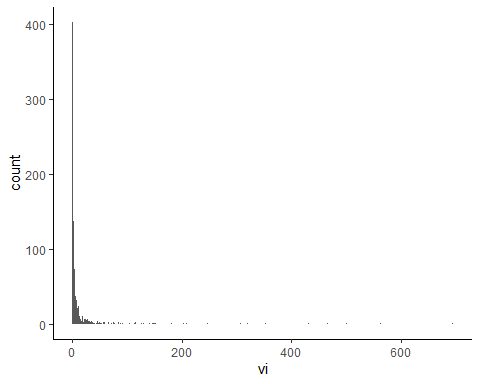
\includegraphics{script-4-meta-analises_files/figure-latex/unnamed-chunk-11-1.pdf}

Comparacoes com vi maior ou igual a 1000: 7 Comparacoes com vi maior ou
igual a 500 (e menor que 1000): 3 Comparacoes com vi maior ou igual a
100 (e menor que 500): 21 Comparacoes com vi maior ou igual a 50 (e
menor que 100): 19 Comparacoes com vi maior ou igual a 10 (e menor que
50): 171

Por enquanto, removemos comparacoes com variancia igual ou maior que
1000.

\begin{verbatim}
## 
## Random-Effects Model (k = 1181; tau^2 estimator: REML)
## 
##     logLik    deviance         AIC         BIC        AICc   
## -3709.6779   7419.3558   7423.3558   7433.5023   7423.3660   
## 
## tau^2 (estimated amount of total heterogeneity): 12.8842 (SE = 0.6661)
## tau (square root of estimated tau^2 value):      3.5895
## I^2 (total heterogeneity / total variability):   92.11%
## H^2 (total variability / sampling variability):  12.67
## 
## Test for Heterogeneity:
## Q(df = 1180) = 7089.4914, p-val < .0001
## 
## Model Results:
## 
## estimate      se      zval    pval    ci.lb    ci.ub      
##  -4.7274  0.1196  -39.5315  <.0001  -4.9618  -4.4930  *** 
## 
## ---
## Signif. codes:  0 '***' 0.001 '**' 0.01 '*' 0.05 '.' 0.1 ' ' 1
\end{verbatim}

\begin{verbatim}
## 
##        estimate   ci.lb   ci.ub 
## tau^2   12.8842 25.1266 33.5264 
## tau      3.5895  5.0126  5.7902 
## I^2(%)  92.1060 95.7903 96.8114 
## H^2     12.6679 23.7546 31.3614
\end{verbatim}

Acho que vale conferir pelo menos os 4 maiores valores de vi, mas talvez
mesmo os outros ainda ficam algumas ordens de grandeza acima dos menores
valores.

Forest plot (SMD)

Meta-análise (3-level SMD)

\begin{verbatim}
## 
## Multivariate Meta-Analysis Model (k = 1181; method: REML)
## 
## Variance Components:
## 
##             estim    sqrt  nlvls  fixed                    factor 
## sigma^2.1  7.6441  2.7648    347     no                rayyan.key 
## sigma^2.2  5.6945  2.3863   1181     no  rayyan.key/Comparison.ID 
## 
## Test for Heterogeneity:
## Q(df = 1180) = 7089.4914, p-val < .0001
## 
## Model Results:
## 
## estimate      se      zval    pval    ci.lb    ci.ub      
##  -5.3505  0.1925  -27.7883  <.0001  -5.7279  -4.9731  *** 
## 
## ---
## Signif. codes:  0 '***' 0.001 '**' 0.01 '*' 0.05 '.' 0.1 ' ' 1
\end{verbatim}

\begin{verbatim}
## $results
##               % of total variance    I2
## Level 1                  7.645608   ---
## Level 2 (exp)           39.427587 39.43
## Level 3 (art)           52.926805 52.93
## 
## $totalI2
## [1] 92.35439
## 
## $plot
\end{verbatim}

\begin{verbatim}
## 
## attr(,"class")
## [1] "mlm.variance.distribution" "list"
\end{verbatim}

Trim-and-fill (only for 2-level model)

Funnel plot
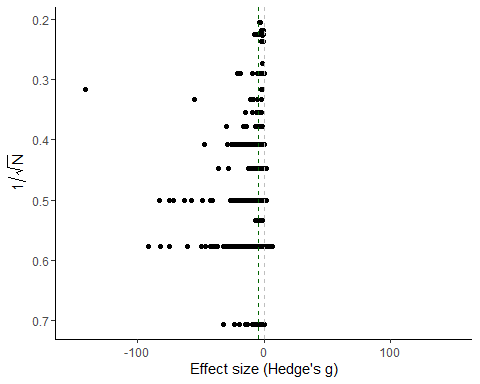
\includegraphics{script-4-meta-analises_files/figure-latex/unnamed-chunk-18-1.pdf}

\begin{verbatim}
## Saving 6.5 x 4.5 in image
\end{verbatim}

Egger's regression

\begin{verbatim}
## 
## Regression Test for Funnel Plot Asymmetry
## 
## Model:     mixed-effects meta-regression model
## Predictor: inverse of the square root sample size
## 
## Test for Funnel Plot Asymmetry: z = -2.4982, p = 0.0125
## Limit Estimate (as ni -> inf):  b = -3.1152 (CI: -4.3989, -1.8316)
\end{verbatim}

Meta-regressions (3-level)

Differentiation

\begin{verbatim}
## Warning: Rows with NAs omitted from model fitting.
\end{verbatim}

\begin{verbatim}
## 
## Multivariate Meta-Analysis Model (k = 1155; method: REML)
## 
## Variance Components:
## 
##             estim    sqrt  nlvls  fixed                    factor 
## sigma^2.1  7.5849  2.7541    345     no                rayyan.key 
## sigma^2.2  5.5024  2.3457   1155     no  rayyan.key/Comparison.ID 
## 
## Test for Residual Heterogeneity:
## QE(df = 1151) = 6887.5576, p-val < .0001
## 
## Test of Moderators (coefficients 2:4):
## QM(df = 3) = 2.4731, p-val = 0.4802
## 
## Model Results:
## 
##                                                                                             estimate 
## intrcpt                                                                                      -5.4822 
## relevel(factor(dados_meta_smd$Diferentiation_method), ref = "No differentiation")ATRA         0.5599 
## relevel(factor(dados_meta_smd$Diferentiation_method), ref = "No differentiation")ATRA plus    0.9769 
## relevel(factor(dados_meta_smd$Diferentiation_method), ref = "No differentiation")Other        0.3227 
##                                                                                                 se 
## intrcpt                                                                                     0.2095 
## relevel(factor(dados_meta_smd$Diferentiation_method), ref = "No differentiation")ATRA       0.5397 
## relevel(factor(dados_meta_smd$Diferentiation_method), ref = "No differentiation")ATRA plus  0.7807 
## relevel(factor(dados_meta_smd$Diferentiation_method), ref = "No differentiation")Other      1.3498 
##                                                                                                 zval 
## intrcpt                                                                                     -26.1705 
## relevel(factor(dados_meta_smd$Diferentiation_method), ref = "No differentiation")ATRA         1.0375 
## relevel(factor(dados_meta_smd$Diferentiation_method), ref = "No differentiation")ATRA plus    1.2512 
## relevel(factor(dados_meta_smd$Diferentiation_method), ref = "No differentiation")Other        0.2391 
##                                                                                               pval 
## intrcpt                                                                                     <.0001 
## relevel(factor(dados_meta_smd$Diferentiation_method), ref = "No differentiation")ATRA       0.2995 
## relevel(factor(dados_meta_smd$Diferentiation_method), ref = "No differentiation")ATRA plus  0.2109 
## relevel(factor(dados_meta_smd$Diferentiation_method), ref = "No differentiation")Other      0.8110 
##                                                                                               ci.lb 
## intrcpt                                                                                     -5.8927 
## relevel(factor(dados_meta_smd$Diferentiation_method), ref = "No differentiation")ATRA       -0.4978 
## relevel(factor(dados_meta_smd$Diferentiation_method), ref = "No differentiation")ATRA plus  -0.5533 
## relevel(factor(dados_meta_smd$Diferentiation_method), ref = "No differentiation")Other      -2.3228 
##                                                                                               ci.ub 
## intrcpt                                                                                     -5.0716 
## relevel(factor(dados_meta_smd$Diferentiation_method), ref = "No differentiation")ATRA        1.6176 
## relevel(factor(dados_meta_smd$Diferentiation_method), ref = "No differentiation")ATRA plus   2.5071 
## relevel(factor(dados_meta_smd$Diferentiation_method), ref = "No differentiation")Other       2.9682 
##                                                                                                 
## intrcpt                                                                                     *** 
## relevel(factor(dados_meta_smd$Diferentiation_method), ref = "No differentiation")ATRA           
## relevel(factor(dados_meta_smd$Diferentiation_method), ref = "No differentiation")ATRA plus      
## relevel(factor(dados_meta_smd$Diferentiation_method), ref = "No differentiation")Other          
## 
## ---
## Signif. codes:  0 '***' 0.001 '**' 0.01 '*' 0.05 '.' 0.1 ' ' 1
\end{verbatim}

Differentiation bubble plot

\begin{verbatim}
## Warning in geom_abline(yintercept = 0, slope = 0, linetype = "dashed", color =
## "grey"): Ignoring unknown parameters: `yintercept`
\end{verbatim}

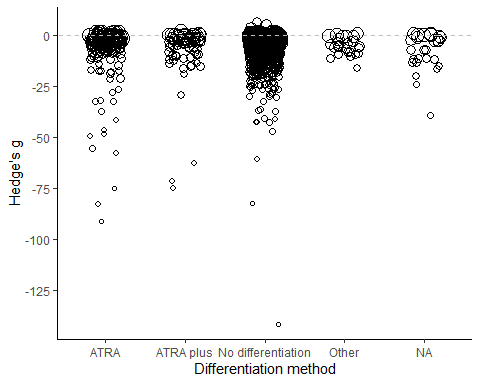
\includegraphics{script-4-meta-analises_files/figure-latex/unnamed-chunk-21-1.pdf}

Diff. duration

\begin{verbatim}
## Warning: Rows with NAs omitted from model fitting.
\end{verbatim}

\begin{verbatim}
## 
## Multivariate Meta-Analysis Model (k = 385; method: REML)
## 
## Variance Components:
## 
##              estim    sqrt  nlvls  fixed                    factor 
## sigma^2.1  17.0264  4.1263    105     no                rayyan.key 
## sigma^2.2   3.3697  1.8357    385     no  rayyan.key/Comparison.ID 
## 
## Test for Residual Heterogeneity:
## QE(df = 383) = 2177.3348, p-val < .0001
## 
## Test of Moderators (coefficient 2):
## QM(df = 1) = 3.0267, p-val = 0.0819
## 
## Model Results:
## 
##                                              estimate      se      zval    pval 
## intrcpt                                       -6.4135  0.5931  -10.8136  <.0001 
## dados_meta_smd$Diferentiation_duration_days    0.1929  0.1109    1.7397  0.0819 
##                                                ci.lb    ci.ub      
## intrcpt                                      -7.5760  -5.2511  *** 
## dados_meta_smd$Diferentiation_duration_days  -0.0244   0.4102    . 
## 
## ---
## Signif. codes:  0 '***' 0.001 '**' 0.01 '*' 0.05 '.' 0.1 ' ' 1
\end{verbatim}

Diff. duration bubble plot

\begin{verbatim}
## Warning: Removed 796 rows containing missing values (`geom_point()`).
\end{verbatim}

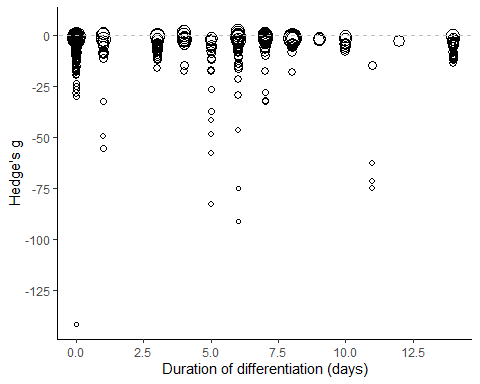
\includegraphics{script-4-meta-analises_files/figure-latex/unnamed-chunk-23-1.pdf}

Aggregation

\begin{verbatim}
## Warning: Rows with NAs omitted from model fitting.
\end{verbatim}

\begin{verbatim}
## 
## Multivariate Meta-Analysis Model (k = 1180; method: REML)
## 
## Variance Components:
## 
##             estim    sqrt  nlvls  fixed                    factor 
## sigma^2.1  7.6454  2.7650    347     no                rayyan.key 
## sigma^2.2  5.5716  2.3604   1180     no  rayyan.key/Comparison.ID 
## 
## Test for Residual Heterogeneity:
## QE(df = 1176) = 6856.7069, p-val < .0001
## 
## Test of Moderators (coefficients 2:4):
## QM(df = 3) = 16.6265, p-val = 0.0008
## 
## Model Results:
## 
##                                                                              estimate 
## intrcpt                                                                       -5.7203 
## relevel(factor(dados_meta_smd$Abeta_aggregation), ref = "Unclear")Fibers      -0.4068 
## relevel(factor(dados_meta_smd$Abeta_aggregation), ref = "Unclear")Monomers     1.7154 
## relevel(factor(dados_meta_smd$Abeta_aggregation), ref = "Unclear")Oligomers    0.8871 
##                                                                                  se 
## intrcpt                                                                      0.2566 
## relevel(factor(dados_meta_smd$Abeta_aggregation), ref = "Unclear")Fibers     0.5387 
## relevel(factor(dados_meta_smd$Abeta_aggregation), ref = "Unclear")Monomers   0.6080 
## relevel(factor(dados_meta_smd$Abeta_aggregation), ref = "Unclear")Oligomers  0.3660 
##                                                                                  zval 
## intrcpt                                                                      -22.2893 
## relevel(factor(dados_meta_smd$Abeta_aggregation), ref = "Unclear")Fibers      -0.7553 
## relevel(factor(dados_meta_smd$Abeta_aggregation), ref = "Unclear")Monomers     2.8213 
## relevel(factor(dados_meta_smd$Abeta_aggregation), ref = "Unclear")Oligomers    2.4238 
##                                                                                pval 
## intrcpt                                                                      <.0001 
## relevel(factor(dados_meta_smd$Abeta_aggregation), ref = "Unclear")Fibers     0.4501 
## relevel(factor(dados_meta_smd$Abeta_aggregation), ref = "Unclear")Monomers   0.0048 
## relevel(factor(dados_meta_smd$Abeta_aggregation), ref = "Unclear")Oligomers  0.0154 
##                                                                                ci.lb 
## intrcpt                                                                      -6.2233 
## relevel(factor(dados_meta_smd$Abeta_aggregation), ref = "Unclear")Fibers     -1.4626 
## relevel(factor(dados_meta_smd$Abeta_aggregation), ref = "Unclear")Monomers    0.5237 
## relevel(factor(dados_meta_smd$Abeta_aggregation), ref = "Unclear")Oligomers   0.1698 
##                                                                                ci.ub 
## intrcpt                                                                      -5.2173 
## relevel(factor(dados_meta_smd$Abeta_aggregation), ref = "Unclear")Fibers      0.6489 
## relevel(factor(dados_meta_smd$Abeta_aggregation), ref = "Unclear")Monomers    2.9071 
## relevel(factor(dados_meta_smd$Abeta_aggregation), ref = "Unclear")Oligomers   1.6045 
##                                                                                  
## intrcpt                                                                      *** 
## relevel(factor(dados_meta_smd$Abeta_aggregation), ref = "Unclear")Fibers         
## relevel(factor(dados_meta_smd$Abeta_aggregation), ref = "Unclear")Monomers    ** 
## relevel(factor(dados_meta_smd$Abeta_aggregation), ref = "Unclear")Oligomers    * 
## 
## ---
## Signif. codes:  0 '***' 0.001 '**' 0.01 '*' 0.05 '.' 0.1 ' ' 1
\end{verbatim}

Aggregation bubble plot

\begin{verbatim}
## Warning in geom_abline(yintercept = 0, slope = 0, linetype = "dashed", color =
## "grey"): Ignoring unknown parameters: `yintercept`
\end{verbatim}

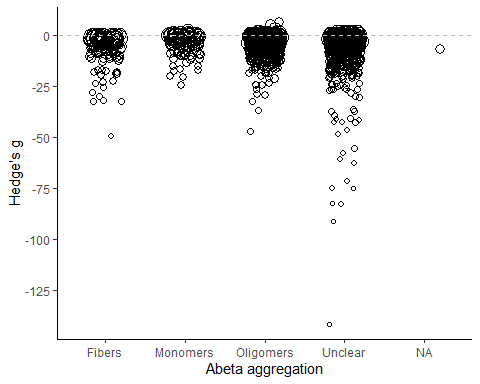
\includegraphics{script-4-meta-analises_files/figure-latex/unnamed-chunk-25-1.pdf}

Abeta concentration

\begin{verbatim}
## 
## Multivariate Meta-Analysis Model (k = 1133; method: REML)
## 
## Variance Components:
## 
##             estim    sqrt  nlvls  fixed                    factor 
## sigma^2.1  7.5742  2.7521    339     no                rayyan.key 
## sigma^2.2  5.7816  2.4045   1133     no  rayyan.key/Comparison.ID 
## 
## Test for Residual Heterogeneity:
## QE(df = 1131) = 6817.5402, p-val < .0001
## 
## Test of Moderators (coefficient 2):
## QM(df = 1) = 0.8983, p-val = 0.3432
## 
## Model Results:
## 
##                                          estimate      se      zval    pval 
## intrcpt                                   -5.3132  0.1946  -27.2990  <.0001 
## dados_meta_smd_max2500$Concentration_uM   -0.0006  0.0006   -0.9478  0.3432 
##                                            ci.lb    ci.ub      
## intrcpt                                  -5.6946  -4.9317  *** 
## dados_meta_smd_max2500$Concentration_uM  -0.0018   0.0006      
## 
## ---
## Signif. codes:  0 '***' 0.001 '**' 0.01 '*' 0.05 '.' 0.1 ' ' 1
\end{verbatim}

Abeta concentration bubble plot
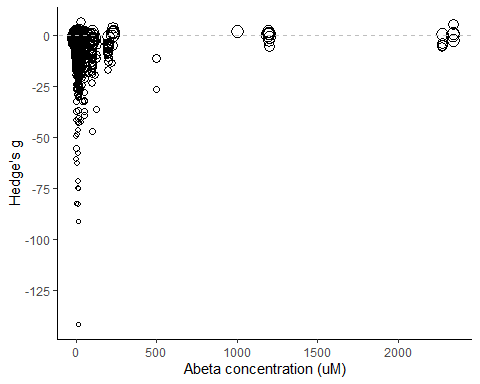
\includegraphics{script-4-meta-analises_files/figure-latex/unnamed-chunk-27-1.pdf}

Abeta duration of exposure

\begin{verbatim}
## Warning: Rows with NAs omitted from model fitting.
\end{verbatim}

\begin{verbatim}
## 
## Multivariate Meta-Analysis Model (k = 1170; method: REML)
## 
## Variance Components:
## 
##             estim    sqrt  nlvls  fixed                    factor 
## sigma^2.1  7.8467  2.8012    341     no                rayyan.key 
## sigma^2.2  5.5477  2.3553   1170     no  rayyan.key/Comparison.ID 
## 
## Test for Residual Heterogeneity:
## QE(df = 1168) = 7035.6290, p-val < .0001
## 
## Test of Moderators (coefficient 2):
## QM(df = 1) = 15.8005, p-val < .0001
## 
## Model Results:
## 
##                                            estimate      se      zval    pval 
## intrcpt                                     -4.2544  0.3417  -12.4513  <.0001 
## as.numeric(dados_meta_smd$Duration_hours)   -0.0344  0.0087   -3.9750  <.0001 
##                                              ci.lb    ci.ub      
## intrcpt                                    -4.9240  -3.5847  *** 
## as.numeric(dados_meta_smd$Duration_hours)  -0.0513  -0.0174  *** 
## 
## ---
## Signif. codes:  0 '***' 0.001 '**' 0.01 '*' 0.05 '.' 0.1 ' ' 1
\end{verbatim}

Abeta duration bubble plot

\begin{verbatim}
## Warning: Removed 11 rows containing missing values (`geom_point()`).
\end{verbatim}

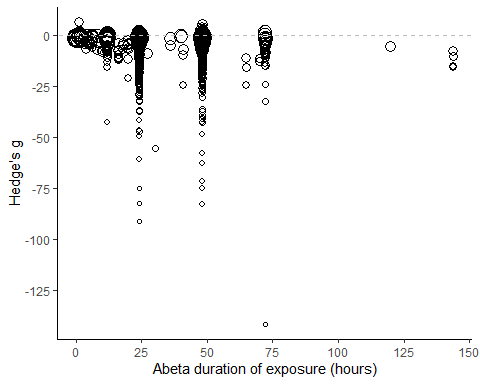
\includegraphics{script-4-meta-analises_files/figure-latex/unnamed-chunk-29-1.pdf}

Assay

\begin{verbatim}
## Warning: Rows with NAs omitted from model fitting.
\end{verbatim}

\begin{verbatim}
## 
## Multivariate Meta-Analysis Model (k = 1174; method: REML)
## 
## Variance Components:
## 
##             estim    sqrt  nlvls  fixed                    factor 
## sigma^2.1  7.6762  2.7706    346     no                rayyan.key 
## sigma^2.2  5.8285  2.4142   1174     no  rayyan.key/Comparison.ID 
## 
## Test for Residual Heterogeneity:
## QE(df = 1167) = 6990.8863, p-val < .0001
## 
## Test of Moderators (coefficients 2:7):
## QM(df = 6) = 4.0302, p-val = 0.6726
## 
## Model Results:
## 
##                                                            estimate      se 
## intrcpt                                                     -5.4786  0.2127 
## relevel(factor(dados_meta_smd$Assay), ref = "MTT")CCK-8      0.0243  0.9831 
## relevel(factor(dados_meta_smd$Assay), ref = "MTT")EZ4U      -0.1948  3.0309 
## relevel(factor(dados_meta_smd$Assay), ref = "MTT")MTS       -0.2966  1.0399 
## relevel(factor(dados_meta_smd$Assay), ref = "MTT")MTS/PMS    4.0511  3.7374 
## relevel(factor(dados_meta_smd$Assay), ref = "MTT")WST        1.2240  0.7539 
## relevel(factor(dados_meta_smd$Assay), ref = "MTT")XTT        0.6081  1.5798 
##                                                                zval    pval 
## intrcpt                                                    -25.7535  <.0001 
## relevel(factor(dados_meta_smd$Assay), ref = "MTT")CCK-8      0.0247  0.9803 
## relevel(factor(dados_meta_smd$Assay), ref = "MTT")EZ4U      -0.0643  0.9488 
## relevel(factor(dados_meta_smd$Assay), ref = "MTT")MTS       -0.2852  0.7755 
## relevel(factor(dados_meta_smd$Assay), ref = "MTT")MTS/PMS    1.0839  0.2784 
## relevel(factor(dados_meta_smd$Assay), ref = "MTT")WST        1.6236  0.1045 
## relevel(factor(dados_meta_smd$Assay), ref = "MTT")XTT        0.3849  0.7003 
##                                                              ci.lb    ci.ub 
## intrcpt                                                    -5.8955  -5.0616 
## relevel(factor(dados_meta_smd$Assay), ref = "MTT")CCK-8    -1.9026   1.9512 
## relevel(factor(dados_meta_smd$Assay), ref = "MTT")EZ4U     -6.1353   5.7458 
## relevel(factor(dados_meta_smd$Assay), ref = "MTT")MTS      -2.3347   1.7415 
## relevel(factor(dados_meta_smd$Assay), ref = "MTT")MTS/PMS  -3.2740  11.3763 
## relevel(factor(dados_meta_smd$Assay), ref = "MTT")WST      -0.2536   2.7015 
## relevel(factor(dados_meta_smd$Assay), ref = "MTT")XTT      -2.4883   3.7045 
##                                                                
## intrcpt                                                    *** 
## relevel(factor(dados_meta_smd$Assay), ref = "MTT")CCK-8        
## relevel(factor(dados_meta_smd$Assay), ref = "MTT")EZ4U         
## relevel(factor(dados_meta_smd$Assay), ref = "MTT")MTS          
## relevel(factor(dados_meta_smd$Assay), ref = "MTT")MTS/PMS      
## relevel(factor(dados_meta_smd$Assay), ref = "MTT")WST          
## relevel(factor(dados_meta_smd$Assay), ref = "MTT")XTT          
## 
## ---
## Signif. codes:  0 '***' 0.001 '**' 0.01 '*' 0.05 '.' 0.1 ' ' 1
\end{verbatim}

Assay bubble plot

\begin{verbatim}
## Warning in geom_abline(yintercept = 0, slope = 0, linetype = "dashed", color =
## "grey"): Ignoring unknown parameters: `yintercept`
\end{verbatim}

\includegraphics{script-4-meta-analises_files/figure-latex/unnamed-chunk-31-1.pdf}

Cell density

\begin{verbatim}
## Warning: Rows with NAs omitted from model fitting.
\end{verbatim}

\begin{verbatim}
## 
## Multivariate Meta-Analysis Model (k = 688; method: REML)
## 
## Variance Components:
## 
##             estim    sqrt  nlvls  fixed                    factor 
## sigma^2.1  8.7239  2.9536    202     no                rayyan.key 
## sigma^2.2  6.4217  2.5341    688     no  rayyan.key/Comparison.ID 
## 
## Test for Residual Heterogeneity:
## QE(df = 686) = 4080.6964, p-val < .0001
## 
## Test of Moderators (coefficient 2):
## QM(df = 1) = 0.0120, p-val = 0.9129
## 
## Model Results:
## 
##                                          estimate      se      zval    pval 
## intrcpt                                   -5.7122  0.2748  -20.7904  <.0001 
## as.numeric(dados_meta_smd$Cell_density)    0.0000  0.0000    0.1094  0.9129 
##                                            ci.lb    ci.ub      
## intrcpt                                  -6.2507  -5.1737  *** 
## as.numeric(dados_meta_smd$Cell_density)  -0.0000   0.0000      
## 
## ---
## Signif. codes:  0 '***' 0.001 '**' 0.01 '*' 0.05 '.' 0.1 ' ' 1
\end{verbatim}

Cell density bubble plot

\begin{verbatim}
## Warning: Removed 493 rows containing missing values (`geom_point()`).
\end{verbatim}

\includegraphics{script-4-meta-analises_files/figure-latex/unnamed-chunk-33-1.pdf}

Multivariate Meta-regressions (3-level)

``All combinations of variables from the selected list were tested in
multivariable models, and the best models were ranked by corrected
Akaike Information Criteria (AICc). For each best model selected (for
complete, training and reactivation datasets with 2- and 3-level
analyses), we decomposed the R2 value for each moderator included. For
this, we calculated the mean of the differences between R2 from models
with and without the moderator in all possible orders of moderator
inclusion. Additionally, we performed a Q test of moderators for each
variable (including all dummy variables for each categorical moderator)
to obtain p-values for individual variables.''

Functions to decompose R2 (3-level)

Como a gente só pode usar as comparacoes que tenham a descricao completa
de todas as variáveis testadas, precisamos filtrar os dadose conferir se
seguimos com N suficiente.

Considering all pre-registered variables, we'd have 212 experiments
available (i.e.~969 exclusions due to missing data). As we have 7
variables, we should have at least 70 comparisons - so can use all of
them now. There are 128 possible models.

\begin{verbatim}
## Initialization...
## TASK: Exhaustive screening of candidate set.
## Fitting...
## 
## After 50 models:
## Best model: yi~1+Concentration_uM+Duration_hours
## Crit= 1278.63706083308
## Mean crit= 1307.85636801629
## 
## After 100 models:
## Best model: yi~1+Diferentiation_duration_days+Concentration_uM+Duration_hours
## Crit= 1276.10340652505
## Mean crit= 1304.63066113697
## 
## After 150 models:
## Best model: yi~1+Diferentiation_duration_days+Concentration_uM+Duration_hours
## Crit= 1276.10340652505
## Mean crit= 1301.68238571445
## Completed.
\end{verbatim}

\begin{verbatim}
## glmulti.analysis
## Method: h / Fitting: rma.mv.glmulti / IC used: aicc
## Level: 1 / Marginality: FALSE
## From 128 models:
## Best IC: 1276.10340652505
## Best model:
## [1] "yi ~ 1 + Diferentiation_duration_days + Concentration_uM + Duration_hours"
## Evidence weight: 0.238368590497681
## Worst IC: 1326.56336778678
## 2 models within 2 IC units.
## 16 models to reach 95% of evidence weight.
\end{verbatim}

Decomposing R2 for the best model:

\begin{verbatim}
## [1] "Running models for Diferentiation_duration_days"
## [1] "Running models for Concentration_uM"
## [1] "Running models for Duration_hours"
## [1] "Running models for Cell_density"
\end{verbatim}

Resultados:

\hypertarget{excluindo-outliers-de-concentracao-de-abeta}{%
\subsection{excluindo outliers de concentracao de
abeta:}\label{excluindo-outliers-de-concentracao-de-abeta}}

Como a gente só pode usar as comparacoes que tenham a descricao completa
de todas as variáveis testadas, precisamos filtrar os dadose conferir se
seguimos com N suficiente.

Considering all pre-registered variables, we'd have 212 experiments
available (i.e.~921 exclusions due to missing data). As we have 7
variables, we should have at least 70 comparisons - so can use all of
them now. There are 128 possible models.

Decomposing R2 for the best model:

Resultados:

\hypertarget{controle-de-qualidade-dos-dados}{%
\subsubsection{Controle de qualidade dos
dados}\label{controle-de-qualidade-dos-dados}}

Revisor como moderador

\begin{verbatim}
## 
##                       Created.By   n 
## 1              Adriano Sebollela  33 
## 2              Ana Paula Sampaio  70 
## 3                  Antônio Felix 132 
## 4  Clarissa Franca Dias Carneiro  43 
## 5              Giovanna Nogueira 140 
## 6   Giulia Scarcella Cancelliero 133 
## 7          Glaucia Maria Almeida 135 
## 8             Nathalia Fernandes 120 
## 9              Nathalia Pinheiro 225 
## 10              Samantha Martins 150
\end{verbatim}

\begin{verbatim}
## 
## Multivariate Meta-Analysis Model (k = 1181; method: REML)
## 
## Variance Components:
## 
##             estim    sqrt  nlvls  fixed                    factor 
## sigma^2.1  7.7757  2.7885    347     no                rayyan.key 
## sigma^2.2  5.7257  2.3928   1181     no  rayyan.key/Comparison.ID 
## 
## Test for Residual Heterogeneity:
## QE(df = 1171) = 6902.7371, p-val < .0001
## 
## Test of Moderators (coefficients 2:10):
## QM(df = 9) = 11.3826, p-val = 0.2504
## 
## Model Results:
## 
##                                                                                                     estimate 
## intrcpt                                                                                              -6.1656 
## relevel(factor(dados_meta_smd$Created.By), ref = "Adriano Sebollela")Ana Paula Sampaio                2.2604 
## relevel(factor(dados_meta_smd$Created.By), ref = "Adriano Sebollela")Antônio Felix                    0.9416 
## relevel(factor(dados_meta_smd$Created.By), ref = "Adriano Sebollela")Clarissa Franca Dias Carneiro    0.5366 
## relevel(factor(dados_meta_smd$Created.By), ref = "Adriano Sebollela")Giovanna Nogueira                0.6540 
## relevel(factor(dados_meta_smd$Created.By), ref = "Adriano Sebollela")Giulia Scarcella Cancelliero     0.1406 
## relevel(factor(dados_meta_smd$Created.By), ref = "Adriano Sebollela")Glaucia Maria Almeida            1.3379 
## relevel(factor(dados_meta_smd$Created.By), ref = "Adriano Sebollela")Nathalia Fernandes               1.0378 
## relevel(factor(dados_meta_smd$Created.By), ref = "Adriano Sebollela")Nathalia Pinheiro                1.1981 
## relevel(factor(dados_meta_smd$Created.By), ref = "Adriano Sebollela")Samantha Martins                -0.1735 
##                                                                                                         se 
## intrcpt                                                                                             0.9719 
## relevel(factor(dados_meta_smd$Created.By), ref = "Adriano Sebollela")Ana Paula Sampaio              1.1988 
## relevel(factor(dados_meta_smd$Created.By), ref = "Adriano Sebollela")Antônio Felix                  1.0949 
## relevel(factor(dados_meta_smd$Created.By), ref = "Adriano Sebollela")Clarissa Franca Dias Carneiro  1.2856 
## relevel(factor(dados_meta_smd$Created.By), ref = "Adriano Sebollela")Giovanna Nogueira              1.1309 
## relevel(factor(dados_meta_smd$Created.By), ref = "Adriano Sebollela")Giulia Scarcella Cancelliero   1.1224 
## relevel(factor(dados_meta_smd$Created.By), ref = "Adriano Sebollela")Glaucia Maria Almeida          1.1159 
## relevel(factor(dados_meta_smd$Created.By), ref = "Adriano Sebollela")Nathalia Fernandes             1.1765 
## relevel(factor(dados_meta_smd$Created.By), ref = "Adriano Sebollela")Nathalia Pinheiro              1.1208 
## relevel(factor(dados_meta_smd$Created.By), ref = "Adriano Sebollela")Samantha Martins               1.1162 
##                                                                                                        zval 
## intrcpt                                                                                             -6.3439 
## relevel(factor(dados_meta_smd$Created.By), ref = "Adriano Sebollela")Ana Paula Sampaio               1.8855 
## relevel(factor(dados_meta_smd$Created.By), ref = "Adriano Sebollela")Antônio Felix                   0.8599 
## relevel(factor(dados_meta_smd$Created.By), ref = "Adriano Sebollela")Clarissa Franca Dias Carneiro   0.4174 
## relevel(factor(dados_meta_smd$Created.By), ref = "Adriano Sebollela")Giovanna Nogueira               0.5783 
## relevel(factor(dados_meta_smd$Created.By), ref = "Adriano Sebollela")Giulia Scarcella Cancelliero    0.1253 
## relevel(factor(dados_meta_smd$Created.By), ref = "Adriano Sebollela")Glaucia Maria Almeida           1.1990 
## relevel(factor(dados_meta_smd$Created.By), ref = "Adriano Sebollela")Nathalia Fernandes              0.8820 
## relevel(factor(dados_meta_smd$Created.By), ref = "Adriano Sebollela")Nathalia Pinheiro               1.0689 
## relevel(factor(dados_meta_smd$Created.By), ref = "Adriano Sebollela")Samantha Martins               -0.1555 
##                                                                                                       pval 
## intrcpt                                                                                             <.0001 
## relevel(factor(dados_meta_smd$Created.By), ref = "Adriano Sebollela")Ana Paula Sampaio              0.0594 
## relevel(factor(dados_meta_smd$Created.By), ref = "Adriano Sebollela")Antônio Felix                  0.3898 
## relevel(factor(dados_meta_smd$Created.By), ref = "Adriano Sebollela")Clarissa Franca Dias Carneiro  0.6764 
## relevel(factor(dados_meta_smd$Created.By), ref = "Adriano Sebollela")Giovanna Nogueira              0.5631 
## relevel(factor(dados_meta_smd$Created.By), ref = "Adriano Sebollela")Giulia Scarcella Cancelliero   0.9003 
## relevel(factor(dados_meta_smd$Created.By), ref = "Adriano Sebollela")Glaucia Maria Almeida          0.2305 
## relevel(factor(dados_meta_smd$Created.By), ref = "Adriano Sebollela")Nathalia Fernandes             0.3778 
## relevel(factor(dados_meta_smd$Created.By), ref = "Adriano Sebollela")Nathalia Pinheiro              0.2851 
## relevel(factor(dados_meta_smd$Created.By), ref = "Adriano Sebollela")Samantha Martins               0.8764 
##                                                                                                       ci.lb 
## intrcpt                                                                                             -8.0705 
## relevel(factor(dados_meta_smd$Created.By), ref = "Adriano Sebollela")Ana Paula Sampaio              -0.0892 
## relevel(factor(dados_meta_smd$Created.By), ref = "Adriano Sebollela")Antônio Felix                  -1.2044 
## relevel(factor(dados_meta_smd$Created.By), ref = "Adriano Sebollela")Clarissa Franca Dias Carneiro  -1.9830 
## relevel(factor(dados_meta_smd$Created.By), ref = "Adriano Sebollela")Giovanna Nogueira              -1.5626 
## relevel(factor(dados_meta_smd$Created.By), ref = "Adriano Sebollela")Giulia Scarcella Cancelliero   -2.0593 
## relevel(factor(dados_meta_smd$Created.By), ref = "Adriano Sebollela")Glaucia Maria Almeida          -0.8492 
## relevel(factor(dados_meta_smd$Created.By), ref = "Adriano Sebollela")Nathalia Fernandes             -1.2682 
## relevel(factor(dados_meta_smd$Created.By), ref = "Adriano Sebollela")Nathalia Pinheiro              -0.9987 
## relevel(factor(dados_meta_smd$Created.By), ref = "Adriano Sebollela")Samantha Martins               -2.3612 
##                                                                                                       ci.ub 
## intrcpt                                                                                             -4.2607 
## relevel(factor(dados_meta_smd$Created.By), ref = "Adriano Sebollela")Ana Paula Sampaio               4.6101 
## relevel(factor(dados_meta_smd$Created.By), ref = "Adriano Sebollela")Antônio Felix                   3.0876 
## relevel(factor(dados_meta_smd$Created.By), ref = "Adriano Sebollela")Clarissa Franca Dias Carneiro   3.0563 
## relevel(factor(dados_meta_smd$Created.By), ref = "Adriano Sebollela")Giovanna Nogueira               2.8705 
## relevel(factor(dados_meta_smd$Created.By), ref = "Adriano Sebollela")Giulia Scarcella Cancelliero    2.3406 
## relevel(factor(dados_meta_smd$Created.By), ref = "Adriano Sebollela")Glaucia Maria Almeida           3.5250 
## relevel(factor(dados_meta_smd$Created.By), ref = "Adriano Sebollela")Nathalia Fernandes              3.3437 
## relevel(factor(dados_meta_smd$Created.By), ref = "Adriano Sebollela")Nathalia Pinheiro               3.3948 
## relevel(factor(dados_meta_smd$Created.By), ref = "Adriano Sebollela")Samantha Martins                2.0141 
##                                                                                                         
## intrcpt                                                                                             *** 
## relevel(factor(dados_meta_smd$Created.By), ref = "Adriano Sebollela")Ana Paula Sampaio                . 
## relevel(factor(dados_meta_smd$Created.By), ref = "Adriano Sebollela")Antônio Felix                      
## relevel(factor(dados_meta_smd$Created.By), ref = "Adriano Sebollela")Clarissa Franca Dias Carneiro      
## relevel(factor(dados_meta_smd$Created.By), ref = "Adriano Sebollela")Giovanna Nogueira                  
## relevel(factor(dados_meta_smd$Created.By), ref = "Adriano Sebollela")Giulia Scarcella Cancelliero       
## relevel(factor(dados_meta_smd$Created.By), ref = "Adriano Sebollela")Glaucia Maria Almeida              
## relevel(factor(dados_meta_smd$Created.By), ref = "Adriano Sebollela")Nathalia Fernandes                 
## relevel(factor(dados_meta_smd$Created.By), ref = "Adriano Sebollela")Nathalia Pinheiro                  
## relevel(factor(dados_meta_smd$Created.By), ref = "Adriano Sebollela")Samantha Martins                   
## 
## ---
## Signif. codes:  0 '***' 0.001 '**' 0.01 '*' 0.05 '.' 0.1 ' ' 1
\end{verbatim}

\begin{verbatim}
## Warning in geom_abline(yintercept = 0, slope = 0, linetype = "dashed", color =
## "grey"): Ignoring unknown parameters: `yintercept`
\end{verbatim}

\includegraphics{script-4-meta-analises_files/figure-latex/unnamed-chunk-46-1.pdf}

\hypertarget{anuxe1lises-descritivas}{%
\subsubsection{Análises descritivas}\label{anuxe1lises-descritivas}}

\includegraphics{script-4-meta-analises_files/figure-latex/unnamed-chunk-48-1.pdf}

Article-level info:

\begin{longtable}[]{@{}lrr@{}}
\toprule()
Feature & Count & Percent \\
\midrule()
\endhead
Studies testing reversal & 245 & 69.4 \\
Provides sample size calculation & 0 & 0.0 \\
Includes conflict of interest statement & 180 & 51.0 \\
Has pre-registered & 10 & 2.8 \\
\bottomrule()
\end{longtable}

Experiment-level info

Assay

\begin{longtable}[]{@{}lr@{}}
\toprule()
Assay & n \\
\midrule()
\endhead
MTT & 1007 \\
WST & 81 \\
CCK-8 & 51 \\
MTS & 30 \\
XTT & 15 \\
NA & 7 \\
EZ4U & 2 \\
MTS/PMS & 1 \\
\bottomrule()
\end{longtable}

Cell line

\begin{longtable}[]{@{}lr@{}}
\toprule()
Cell\_source & n \\
\midrule()
\endhead
Cell bank & 637 \\
Unclear & 475 \\
Donation & 82 \\
\bottomrule()
\end{longtable}

\begin{longtable}[]{@{}
  >{\raggedright\arraybackslash}p{(\columnwidth - 2\tabcolsep) * \real{0.9545}}
  >{\raggedleft\arraybackslash}p{(\columnwidth - 2\tabcolsep) * \real{0.0455}}@{}}
\toprule()
\begin{minipage}[b]{\linewidth}\raggedright
Cell\_bank
\end{minipage} & \begin{minipage}[b]{\linewidth}\raggedleft
n
\end{minipage} \\
\midrule()
\endhead
American Type Culture Collection (ATCC) & 293 \\
European Collection of Authenticated Cell Cultures (ECACC) & 192 \\
Chinese Academy of Sciences & 44 \\
Leibniz Institute DSMZ - German Collection of Microorganisms and Cell
Cultures GmbH & 29 \\
Riken Cell Bank & 28 \\
National Centre for Cell Science (NCCS) & 15 \\
Sigma-Aldrich & 8 \\
Institute of Biochemistry and Cell Biology & 7 \\
Invitrogen & 5 \\
Pasteur Institute of Iran & 5 \\
Korean Cell Line Bank & 4 \\
NA & 3 \\
cells were purchased from Zhong Qiao Xin Zhou Biotec Co., Ltd (Shanghai,
China) & 2 \\
LGC Promo-chem & 1 \\
The Cell Resource Centre of Institute of Basic Medicine & 1 \\
\bottomrule()
\end{longtable}

\begin{longtable}[]{@{}lr@{}}
\toprule()
Cell\_authentication & n \\
\midrule()
\endhead
No & 1171 \\
Yes, no protocol & 17 \\
NA & 6 \\
\bottomrule()
\end{longtable}

\begin{longtable}[]{@{}lr@{}}
\toprule()
Cell\_mycoplasma & n \\
\midrule()
\endhead
No & 1170 \\
Yes, no protocol & 18 \\
NA & 6 \\
\bottomrule()
\end{longtable}

\begin{longtable}[]{@{}lr@{}}
\toprule()
Serum\_type & n \\
\midrule()
\endhead
FBS & 758 \\
FCS & 233 \\
Unclear & 195 \\
FBS and HS & 3 \\
CS & 2 \\
FCS and FHS & 1 \\
FCS and HS & 1 \\
NO SERUM & 1 \\
\bottomrule()
\end{longtable}

\begin{longtable}[]{@{}lr@{}}
\toprule()
Serum\_concentration & n \\
\midrule()
\endhead
0.1 & 750 \\
0.15 & 205 \\
NA & 202 \\
0.05 & 7 \\
0.18 & 7 \\
0.17 & 6 \\
0.2 & 5 \\
0.02 & 4 \\
5\% of each & 3 \\
5\% or 10 \% & 2 \\
0.12 & 1 \\
10\% and 5\% & 1 \\
5\% and 10\% & 1 \\
\bottomrule()
\end{longtable}

Treatment

\begin{longtable}[]{@{}lr@{}}
\toprule()
Control\_description & n \\
\midrule()
\endhead
Unclear & 510 \\
Vehicle & 343 \\
Medium only & 300 \\
Other & 41 \\
\bottomrule()
\end{longtable}

\begin{longtable}[]{@{}lr@{}}
\toprule()
Abeta\_sequence & n \\
\midrule()
\endhead
1-42 & 964 \\
1-40 & 218 \\
1-43 & 10 \\
1-38 & 2 \\
\bottomrule()
\end{longtable}

\begin{longtable}[]{@{}lr@{}}
\toprule()
Abeta\_origin & n \\
\midrule()
\endhead
Unclear & 613 \\
synthetic & 523 \\
recombinant & 58 \\
\bottomrule()
\end{longtable}

\begin{longtable}[]{@{}lr@{}}
\toprule()
Abeta\_species & n \\
\midrule()
\endhead
Unclear & 964 \\
Human & 225 \\
Rat & 5 \\
\bottomrule()
\end{longtable}

\begin{longtable}[]{@{}lr@{}}
\toprule()
Abeta\_aggregation & n \\
\midrule()
\endhead
Unclear & 544 \\
Oligomers & 460 \\
Fibers & 101 \\
Monomers & 88 \\
NA & 1 \\
\bottomrule()
\end{longtable}

\begin{longtable}[]{@{}lr@{}}
\toprule()
Single\_exposure & n \\
\midrule()
\endhead
Yes, single & 1192 \\
Unclear & 1 \\
NA & 1 \\
\bottomrule()
\end{longtable}

\begin{verbatim}
## # A tibble: 1 x 1
##   `mean(Duration_hours, na.rm = T)`
##                               <dbl>
## 1                              33.3
\end{verbatim}

\begin{verbatim}
## # A tibble: 1 x 1
##   `sd(Duration_hours, na.rm = T)`
##                             <dbl>
## 1                            16.9
\end{verbatim}

\begin{verbatim}
## # A tibble: 1 x 1
##   `median(Duration_hours, na.rm = T)`
##                                 <dbl>
## 1                                  24
\end{verbatim}

\begin{verbatim}
## # A tibble: 1 x 1
##   `min(Duration_hours, na.rm = T)`
##                              <dbl>
## 1                                0
\end{verbatim}

\begin{verbatim}
## # A tibble: 1 x 1
##   `max(Duration_hours, na.rm = T)`
##                              <dbl>
## 1                              144
\end{verbatim}

\begin{verbatim}
## Warning: Removed 11 rows containing non-finite values (`stat_bin()`).
\end{verbatim}

\includegraphics{script-4-meta-analises_files/figure-latex/unnamed-chunk-54-1.pdf}

\begin{verbatim}
## # A tibble: 1 x 1
##   `mean(Concentration_uM, na.rm = T)`
##                                 <dbl>
## 1                                516.
\end{verbatim}

\begin{verbatim}
## # A tibble: 1 x 1
##   `sd(Concentration_uM, na.rm = T)`
##                               <dbl>
## 1                             3581.
\end{verbatim}

\begin{verbatim}
## # A tibble: 1 x 1
##   `median(Concentration_uM, na.rm = T)`
##                                   <dbl>
## 1                                    10
\end{verbatim}

\begin{verbatim}
## # A tibble: 1 x 1
##   `min(Concentration_uM, na.rm = T)`
##                                <dbl>
## 1                                  0
\end{verbatim}

\begin{verbatim}
## # A tibble: 1 x 1
##   `max(Concentration_uM, na.rm = T)`
##                                <dbl>
## 1                              46510
\end{verbatim}

\begin{verbatim}
## Warning: Removed 17 rows containing non-finite values (`stat_bin()`).
\end{verbatim}

\includegraphics{script-4-meta-analises_files/figure-latex/unnamed-chunk-55-1.pdf}

Diferenciacao

\begin{longtable}[]{@{}lr@{}}
\toprule()
Diferentiation\_method & n \\
\midrule()
\endhead
No differentiation & 925 \\
ATRA & 151 \\
ATRA plus & 67 \\
NA & 26 \\
Other & 25 \\
\bottomrule()
\end{longtable}

Reporting

\begin{longtable}[]{@{}lrr@{}}
\toprule()
Feature & Count & Percent \\
\midrule()
\endhead
Describes cell source & 719 & 60.2 \\
Describes cell authentication & 17 & 1.4 \\
Describes mycoplasma testing & 18 & 1.5 \\
Control group is clear & 510 & 42.7 \\
Describes Abeta sequence & 1194 & 100.0 \\
Describes Abeta origin & 613 & 51.3 \\
Describes Abeta species & 964 & 80.7 \\
Describes Abeta aggregation & 544 & 45.6 \\
Has single exposure & 1192 & 99.8 \\
Describes duration of Abeta exposure & 1183 & 99.1 \\
Describes concentration of Abeta & 1177 & 98.6 \\
\bottomrule()
\end{longtable}

\end{document}
